\section{Value Function}
\begin{frame}{}
    \LARGE Reinforcement Learning: \textbf{Value Function}
\end{frame}

\begin{frame}{Value Function}
\begin{itemize}
    \item How good is a state?
    \pause
    \item The \textbf{value function} at state s, is the expected cumulative reward from following the policy from state s:
    $$V^{\pi}(s) = \mathbb{E} \left [ \sum_{t \geq 0} \gamma^t r_t \mid s_0=s, \pi \right ]$$
    \item Computing the value function is generally impractical, but we can try
to approximate (learn) it
    \item The benefit is credit assignment: see directly how an action affects
future returns rather than wait for rollouts

\end{itemize}

\end{frame}

\begin{frame}{The Discount Factor $\gamma$}
\begin{itemize}
    \item $\gamma \in [0,1]$ controls how much the agent values future rewards
    \item $\gamma = 0$: agent is completely myopic, only cares about immediate reward
    \item $\gamma \rightarrow 1$: agent values future rewards almost as much as immediate ones
    \item Practical implication: $\gamma = 0.99$ means a reward 100 steps away is worth $\sim$37\% of its face value
    \item Why not $\gamma = 1$? In continuing tasks (no terminal state), the sum of rewards can diverge to infinity, making the objective undefined
    \item Rule of thumb: use $\gamma$ closer to 1 for long-horizon tasks, smaller $\gamma$ for tasks where short-term feedback is reliable
\end{itemize}
\end{frame}

\begin{frame}{Episodic vs.\ Continuing Tasks}
\begin{itemize}
    \item \textbf{Episodic}: interaction breaks into episodes with a clear terminal state (e.g., a chess game ends in win/loss/draw, a robot falls over). Each episode starts fresh from an initial state distribution
    \item \textbf{Continuing}: interaction goes on indefinitely with no natural endpoint (e.g., a stock trading agent, a power grid controller). Discounting is essential here to keep returns finite
    \item Most benchmark environments (CartPole, Atari, MuJoCo) are episodic
    \item This distinction affects how we compute returns and will matter when we derive policy gradient methods on Day 3
\end{itemize}
\end{frame}

\begin{frame}{Value Function}
\begin{figure}
\centering
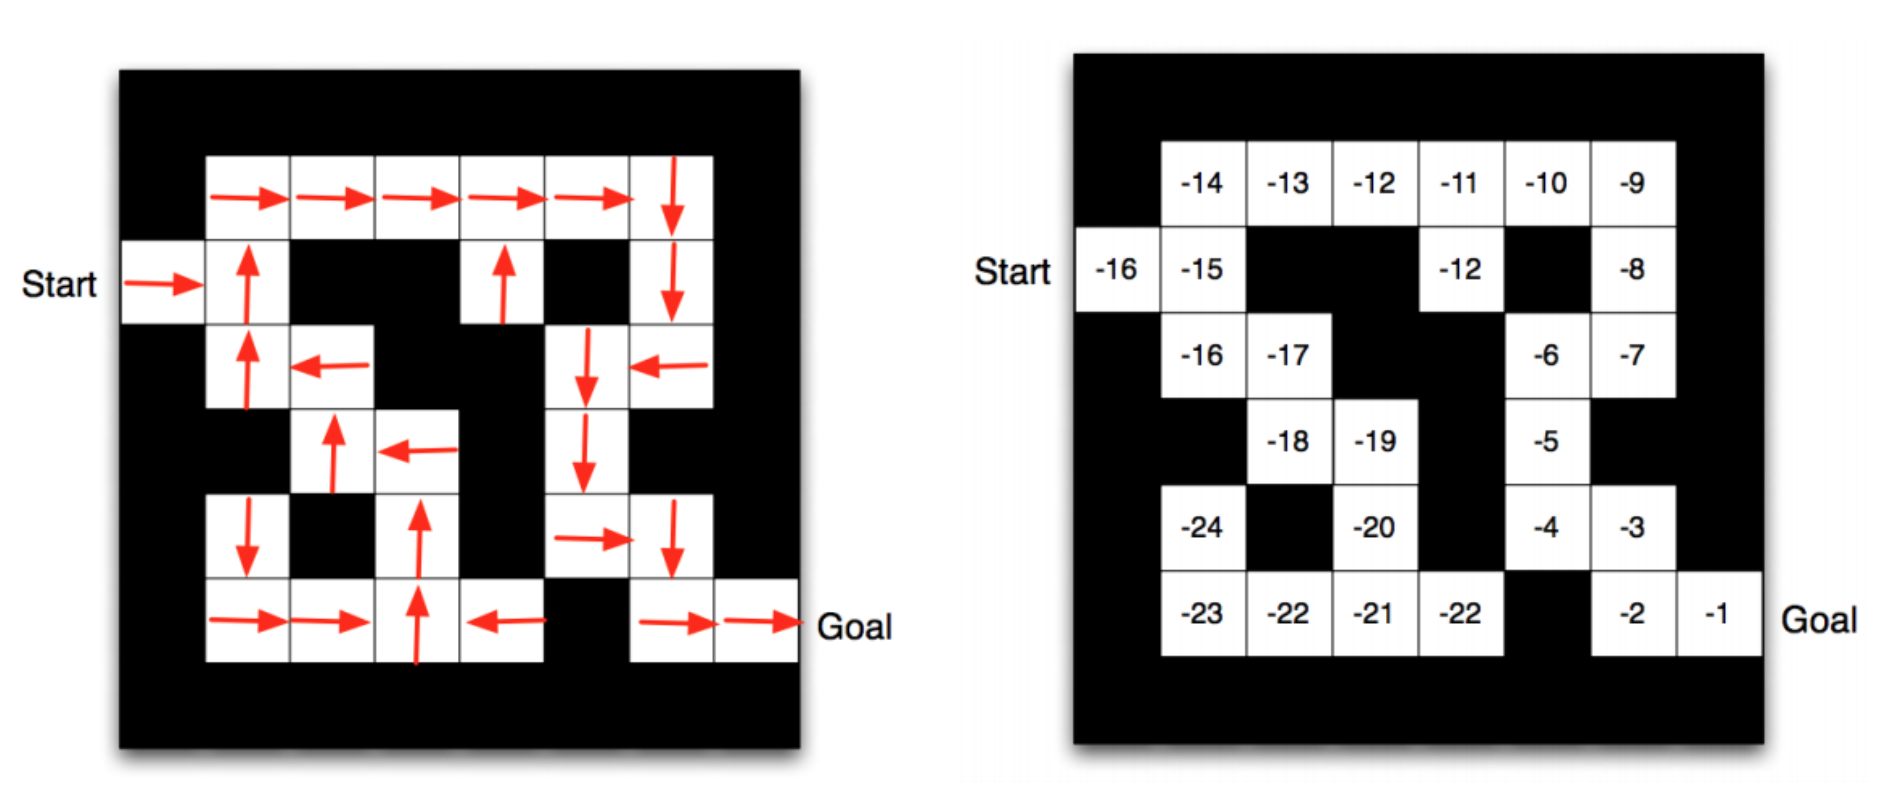
\includegraphics[width=0.9\textwidth,height=0.9\textheight,keepaspectratio]{images/intro/value.png}
\end{figure}

\end{frame}

\section{Q-Value Function}
\begin{frame}{Q-Value Function}
\begin{itemize}
    \item Can we use a value function to choose actions?
    $$\arg \max_a r(s_t,a) + \gamma \mathbb{E}_{p(s_{t+1}|s_t, a_t)}\left [ V^{\pi}(s_{t+1}) \right ]$$
    \pause
    \item \textbf{Problem:} this requires taking the expectation with respect to the environment’s dynamics, which we don’t have direct access to!
    \item Instead, learn a Q-value function.

\end{itemize}
\end{frame}

\begin{frame}{Q-Value Function}
\begin{itemize}
    \item The Q-value function at state s and action a, is the expected cumulative reward from taking action a in state s and then following the policy:
    $$Q^{\pi}(s,a) = \mathbb{E} \left [ \sum_{t \geq 0} \gamma^t r_t \mid s_0=s, a_0=a, \pi \right ]$$
    \item Relationship: $$V^{\pi}(s) = \sum_a \pi(a|s) Q^{\pi}(s,a)$$
    \item Optimal Action: $$\arg \max_a Q^{\pi}(s,a)$$
\end{itemize}
    
\end{frame}

\begin{frame}{The Advantage Function}
\begin{itemize}
    \item Recall: $V^{\pi}(s) = \sum_a \pi(a|s)\, Q^{\pi}(s,a)$
    \item The advantage function measures how much better action $a$ is compared to the average action in state $s$ under policy $\pi$:
    $$A^{\pi}(s,a) = Q^{\pi}(s,a) - V^{\pi}(s)$$
    \item Intuition: if $A^{\pi}(s,a) > 0$, action $a$ is better than what the policy would do on average --- we should do it more
    \item If $A^{\pi}(s,a) < 0$, action $a$ is worse than average --- we should do it less
    \item $A^{\pi}(s,a) = 0$ for all $a$ when the policy is already optimal in that state
    \item This function will be central to Actor-Critic methods on Day 4 and PPO
\end{itemize}
\end{frame}

\section{Bellman Equation}
\begin{frame}{Bellman Equation}
\begin{itemize}
    \item The Bellman Equation is a recursive formula for the Q-value function:
$$Q^{\pi}(s,a) =  r(s,a) + \gamma \mathbb{E}_{p(s'|s, a)\pi(a'|s')}\left [ Q^{\pi}(s',a') \right ]$$
    \item There are various Bellman equations, and most RL algorithms are based on repeatedly applying one of them.
\end{itemize}

\vspace{1em}
\begin{quote}
\small The key insight is that the value of a state can be expressed in terms of the values of the states you might end up in next. This recursion is what makes the Bellman equation powerful --- and computable. You do not need to look infinitely far into the future; you only need to look one step ahead and trust your current value estimate for the rest.
\end{quote}
    
\end{frame}

\begin{frame}{Bellman Equations in Detail}
\begin{itemize}
    \item For the value function $V^{\pi}(s)$:
    $$
    V^{\pi}(s) = \sum_{a} \pi(a|s) \sum_{s'} p(s'|s,a) \left[ r(s,a) + \gamma V^{\pi}(s') \right]
    $$
    \item For the Q-value function $Q^{\pi}(s,a)$:
    $$
    Q^{\pi}(s,a) = \sum_{s'} p(s'|s,a) \left[ r(s,a) + \gamma \sum_{a'} \pi(a'|s') Q^{\pi}(s',a') \right]
    $$
    \item Most RL algorithms are based on repeatedly applying one of these equations.
\end{itemize}
\end{frame}

\subsection{Optimal Bellman Equation}
\begin{frame}{Optimal Bellman Equation}
\begin{itemize}
    \item The optimal policy $\pi^{\star}$ is the one that maximizes the expected discounted reward, and the optimal Q-value function $Q^{\star}$ is the Q-value function for $\pi^{\star}$
    \item The Optimal Bellman Equation gives a recursive formula for $Q^{\star}$:
    $$Q^{\star}(s,a) = r(s,a) + \gamma \mathbb{E}_{p(s'|s, a)}\left [\max_{a'} Q^{\star}(s',a') \right ]$$
    \item This system of equations characterizes the optimal Q-value function. So maybe we can approximate $Q^{\star}$ by trying to solve the optimal Bellman equation!
    \item \textbf{Intuition}: If the optimal state-action values for the next time-step $Q^{\star}(s',a')$ are known, then the optimal strategy is to take the action that maximizes the expected value of $r(s,a) + \gamma Q^{\star}(s',a')$
\end{itemize}
\end{frame}